% Chapter 1

\chapter{Introduction} % Main chapter title

\label{introductionchapter} % For referencing the chapter elsewhere, use \ref{Chapter1} 

\lhead{Chapter 1. \emph{Introduction}} % This is for the header on each page - perhaps a shortened title

%----------------------------------------------------------------------------------------
\section{Background}
Obesity and overweight are currently global health concerns. A systematic review by~\cite{guh2009incidence} concluded that both overweight and obesity are associated with increased incidence of multiple co-morbidities including type 2 diabetes, cancer and cardiovascular diseases (CVD). The number of people who are considered to be either overweight or obese stands to an approximation of  1.3 billion people~\citep{steyn2006chronic}. A survey by~\cite{abegunde:theburden} which included a total of 23 low-income and middle-income countries had projected a loss US\$84 billion of economic production in between 2006 and 2015 from heart disease, stroke, and diabetes alone in the absence of any significant measures put in place to intervene.

Co-morbidities that are associated with obesity are likely to inundate health care systems~\citep{pollak2010s}. At the moment health-care systems have failed to optimally treat chronic conditions such as diabetes due to lack of time to continuously provide  patient  care which is essential in management of chronic conditions~\citep{quinn2008welldoc}. Resources are insufficient to deal with an overwhelming increase in number of patients; hence there has been suggestions emphasizing on moving part of the care to the hands of patients~\citep{aarsand2012mobile}. This need calls for innovative and citizen-centric  interventions to foster lifestyle changes in order to, both prevent or delay onset of chronic conditions in poulations and also supporting of patients in self-management of a chronic conditions in order to reduce the burden on healthcare systems~\citep{korhonen2010personal,aarsand2012mobile,higgins2016smartphone}. There has been a growing number of initiatives by both commercial and research communities in development of wearable sensors and mobile applications that can nudge individuals to eat healthy and increase their level of physical activity~\citep{chen2014healthytogether}. Citizen centric interventions are now possible due to the current advancements in hardware and software technologies which have facilitated creation of opportunities for automation of health self-management processes~\citep{arsand:mobile}. 

One interesting development trend in both academia and industry is the use of mobiles in health. The mobiles have become an effective way for ``just-in time'' delivery of interventions that target psychological processes~\citep{hsu2014persuasive}. These devices are currently omnipresent and people carry them most of the time~\citep{mattila2008mobile}; hence their presence brings a ``kairo factor'' in delivery of interventions that target both health promotion ~\citep{pollak2010s} and persuasion~\citep{hsu2014persuasive}. Smartphone based applications have been rapidly gaining popularity as effective tools to support delivery of personalized health information~\citep{handel2011mhealth}. One of the prevalent adoption of mobile health apps is their use in self-monitoring to augment \emph{cognitive behaviour therapy} - treatment of behaviour in clinical settings~\citep{mattila2008mobile,medynskiy2010salud}. These apps facilitate data collection of one's health parameters through inbuilt tools such as GPS, accelerometer (body activity sensor), etc; hence present an innovative way of monitoring and improving both health and fitness~\citep{higgins2016smartphone}. In order for such tools to support changes in health behaviour and promotion of healthy lifestyle, theory based strategies such gamification (for enhancement of motivation), enabling self-reflection through goal setting and feedback (for improvement of self-efficacy), and SMS reminders are often applied~\citep{consolvo2009goal,cole2010text,hamari2014persuasive,hamari2014does,higgins2016smartphone}. However, such tools have limitations if there were to be utilized in specific contexts. The basis of the research problem for this study was on a limitation that is related to developing world context but can as well scale to a context of developed world. The research problem is as reported below.
\section{Statement of the Problem}
A review by~\cite{higgins2016smartphone} presented evidence that self-monitoring apps can help patients reach their health and fitness goals. Also these apps can support individuals who are not patients to become aware of their behaviours which is an important step towards taking actions that are necessary in living a healthily lifestyle. However, such apps have limitations as they don't support specific interaction models that accommodate sharing of devices and indirect usage. Such mode of interaction are prevalent and relevant in the context of developing world ; hence self-monitoring applications that are designed for direct use may not replicate well to some populations of users~\citep{kaplan2006can,sambasivan2010}, especially in the context of users that face barriers of direct access to user interfaces or technology~\citep{kumar2015mobile}. Typically, self-monitoring apps utilize  specific theory informed motivational affordances in order to enhance engagement of end users but such incentives have been designed only for a direct user as are not supported in a situation of where you have at least two layers of users that consists of an intermediary user who acts as a bridge for an indirect user who is a beneficiary of information in a self-monitoring app. Such a scenario of intermediated technology is shown on Figure \ref{figure:directVSinterm}  which is profoundly explained by~\cite{sambasivan2010} in the perspective of activity theory~\citep{kaptelinin1997activity}, of where in a direct interaction, a computing device or system is an object with an affordance of an activity of which an end user can perform on the object, while in an intermediated interaction there is an addition layer of human interface (intermediary user) responsible for translating intents of a beneficiary user into actions by carrying out activities to a computing device or system on behalf of an indirect user (beneficiary user).
\begin{figure}[htbp]
  \centering
    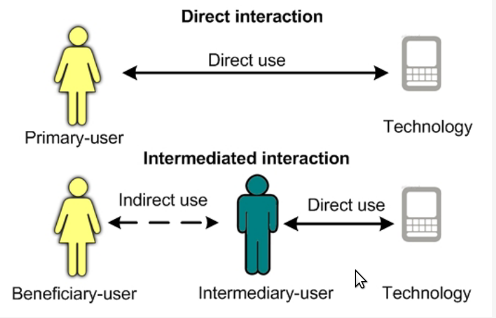
\includegraphics[width=0.6\textwidth]{Figures/intermediated.png}
    \rule{35em}{0.5pt}
  \caption{Direct and intermediated interactions~\citep{sambasivan2010}.}
  \label{figure:directVSinterm}
\end{figure}

This research explored of how one could support a personal health informatics technology of which its usage is facilitated by intermediaries users on behalf of beneficiary users (indirect users). Despite a vast amount of literature on \emph{intermediated technology use}, such persuasive technologies have not been extensively explored in this context. Persuasive technologies tend to have their unique design considerations, and intermediated technology use has its socio-technical aspects; hence one has to understand factors to consider and how to go about implementing a useful intervention that can work in such a complex context. This study had two main research questions as presented below.
\begin{enumerate}
%\setcounter{enumi}{1}
\item What is the role of social-technical settings in intermediated use of gamified self-monitoring application targeting promotion of healthily eating and physical activity?

\textbf{Sub-questions}
\begin{enumerate}[label=\alph*.]
\item What social factors have impact on intermediated use of a gamified self-monitoring application?
\item To what extent those social factors affect motivation to engage with a gamified self-monitoring application in intermediated use context?
\end{enumerate}
\item How gamification plays a role in motivating intermediated use of self-monitoring application targeting promotion of healthily eating and physical activity?

\textbf{Sub-questions}
\begin{enumerate}[label=\alph*.]
\item What is the impact of gamification in supporting self-determination of intermediary users to engage with a self monitoring application in intermediated use context?
\item What is the impact of gamification in supporting self-determination of beneficiary users to engage with a self-monitoring application in intermediated use context?
\item What is the impact of gamification in frequency of utilizing the self-monitoring application in intermediated use context?
\item What is the impact of gamification on motivation of beneficiaries to self monitor diet?
\item What is the impact of gamification on motivation of beneficiaries to self monitor physical activity?
\item How the presence of gamification affects the relationship between an intermediary user and beneficiary user?
\item To what extent gamification may encourage or discourage internalization of intermediated use behaviour?
\end{enumerate}
\end{enumerate}  
\section{Research Contribution}
This research was grounded by user evaluations, ideas from past studies, and  existing theories of human motivation. In total there were three user evaluation studies. These series of user studies were carried out in three townships in South Africa at different intervals of time. Each user study helped to uncover unique insights that were important in getting answers to the aforementioned research questions. Each user study consisted of several pairs of users. Each pair of users consisted one beneficiary user (a person who solicited help in using the self-monitoring application), and one intermediary user (a person who provided needed help to a beneficiary user to facilitate interaction with the self-monitoring application). Beneficiary users elected their respective intermediary users and the pair had access to the app for a certain number of days before questionnaires and interviews were administered.  

Data collection techniques consisted mostly of triangulation of app's usage logs, interviews, and questionnaires. In order to solve the problem, prior to carrying out any prototype development and evaluation, the study kick-started with a contextual investigation to uncover preliminary understanding of users' context through administering semi-structured questionnaire to adult participants who were opportunistically approached in a hospital settings in Cape Town. Contextual investigation was followed by iterations in development and informative evaluations of mobile application prototypes. Motivational affordances implemented on prototypes included gamification features such leader-boards, badges, avatars, virtual pets caring (garden and fish tank), and social interaction features.  Through the course of eliciting feedback from user studies, I as the researcher was able to generate insights in an iterative manner of where each iterative user study informed the formulation and execution of a successive user study. 

From informative evaluations, the study concluded with a summative evaluation which had an objective of measuring the effectiveness of using gamification in promotion of intermediated use in the context of self-monitoring applications. 
 
The contribution of this research is mainly on understanding of social dynamics and motivational affordances to consider when designing a personal health informatics (PHI) for intermediated use. In this dissertation it is suggested that rather than designing a PHI only for the beneficiary alone, one can design for intermediated use, explicitly acknowledging the presence of intermediary user as facilitators of access to a self-monitoring application. This research demonstrated that it is feasible to frame the design of a personal application in way that promotes collaboration between an intermediary user and a beneficiary user; hence reaching the goal of motivating intermediated use. The dissertation highlights some social configurations that are crucial for a self-monitoring application in intermediated use context. The dissertation further emphasizes of the importance of pairing users within family settings to foster an environment that encourage intermediated use.  The study indicated that when a pair consists of immediate family members, then the prior social relationship may promote internalization of help-giving behaviours on the side of intermediaries. Prior social relationship appears to be a prerequisite for setting up an intervention and it can provide rationale for intermediaries to perceive gamification as something that is fun to use but at the same time as something done to support a good cause which in this case it was to help someone you care about. With presence of that care, and by adding a gamification layer,  collaboration and family bonds show indications of improvement, however, in some situations competition appears to harm an existing family bond between members of a pair instead of promoting it especially when one member of a pair feels of being let down by the other member of a pair. Strengths and weaknesses of different motivational affordances in-terms of promoting aspects of autonomy, competence, and relatedness are also discussed in details in order to offer insights to both designers and researchers in designing of future interventions.
\section{Thesis Organization}
The following is an organization of this thesis. Chapter 1 is \emph{\textbf{Introduction}} which provides the background information of the problem, research questions, and lastly the contribution of this research to knowledge. Chapter 2 is \emph{\textbf{Literature Review}} which mainly covers  the theoretical underpinning of this research in terms of related work and the conceptual framework that lays a foundation for this research. Chapter 3 is about \emph{\textbf{Study Context}} which situates this work into South African context by providing a rationale why carrying  a study in South African townships was important. Chapter 4 presents \emph{\textbf{Contextual Enquiry}} that was conducted at the beginning of the study to understand how technology is being utilized in general in the context of older adults who are prospective beneficiary users of the technology. In addition this contextual enquiry aimed to understand if there were particular usage of technology that were health related. Chapter 5 is \emph{\textbf{Prototype I}} of where it describes development and evaluation of the first prototype. Preliminary user requirements used in development of the first prototype were formulated as the results of insights gained from both preliminary findings of the contextual enquiry, and ideas grounded from literature. Chapter 6 is \emph{\textbf{Prototype II}}, this was an improvement of the first prototype. This improvement was as the result of both qualitative feedback from evaluation of the first prototype and researchers' observation of context in the field. Chapter 6 is \emph{\textbf{Summative Evaluation}} of where the second prototype was evaluated with a placebo group to discern the isolated effect of gamification from existing family bonds. Chapter 7 is \emph{\textbf{Conclusion and Future Work}} which discusses how research questions were addressed and highlights reflection from the three evaluation studies by providing insights in terms of design lessons based on strengths and weaknesses of the gamified personalized application for intermediated use. In addition, this last chapter concludes on takeaways from this research and introduces the basis for future research.         
\begin{flushright}
\end{flushright}
